For this part we again used the slide/frame image pairs from assignment 9 to compute homography for several points (instead of the mouse-clicks chosen in Part B) using the RANSAC algorithm. We achieved some meaningful results by doing the following: 

\begin{itemize}
	\item for each slide/frame pair, we used the {\it .sift} files from assignment 9 for SIFT features and created a $M \times 11$ matrix holding the $(x, y)$ coordinates, scale, and direction for video frame image, corresponding $(x, y)$ coordinates, scale, and direction for the slide image, their corresponding Euclidean distance using the nearest neighbor between their 128-element feature vector, angles between their corresponding 128-element feature vector, and Chi-squared measure between their 128-element feature vector. $M$ is the number of features extracted returned by the SIFT. 
	\item we sorted our data matrix by the Euclidean distance and used it as our data set for the RANSAC algorithm, which we ran $k = 178$ times, computed with $n=4$ (number of data points for the model -- need 4 for homography), $w = 0.4$ (the inlier ratio), and $p=0.99$ (the success probability).
	\item for each slide/pair image, we found the best homography $H$, using 4 random rows from the matrix as our inliers, their DLT as our initial model, and then used the frame keypoints from the rest of the data to estimate the slide keypoints. If the RMS between the slide coordinates from the original data matrix and the estimated slide keypoints was within a threshold (chosen as 50), then we included that estimate in our inlier set. 
	\item once the size of the inlier set was over some set value (of $N=150)$, we assumed to have found a good model and recomputed our homography using the DLT with the intial inliers and additional inliers that hold the threshold. 
	\item Fig.~\ref{fig:slideframeC} shows the mapping of keypoints from estimated slide image to the corresponding keypoints on the video frame.  
\end{itemize}

Challenges faced: initally, we had major trouble trying to match the keypoints to reasonable estimated keypoints (going both slide to frame and frame to slide). The estimated keypoints seemed to be in the vicinity of where they should land and by close observation the line often crossed where it supposedly should be... it also looked like the estimated points are bunching up together. After some time-consuming debugging, it turned out there were a couple issues: the RANSAC threshold to decide on the inliers needed reconfiguration and although we were normalizing the estimated keypoints so that the last column of homogenous coordinates was always full of 1s, we were doing it in one line of code and we just had to split them into multiple lines to get the desired results. 

% e double checked and it was not the issue of the visualization, but we also couldn't figure out what's going awry. From the results of Part B), it seems the DLT is working correctly. We also tried decreasing the inlier ratio to increase the number of iterations $k$ for the RANSAC algorithm, but got similar results as shown in Fig.~\ref{fig:slideframeC}. 

\begin{figure}[ht]
	\begin{subfigure}{0.4\textwidth}
	    {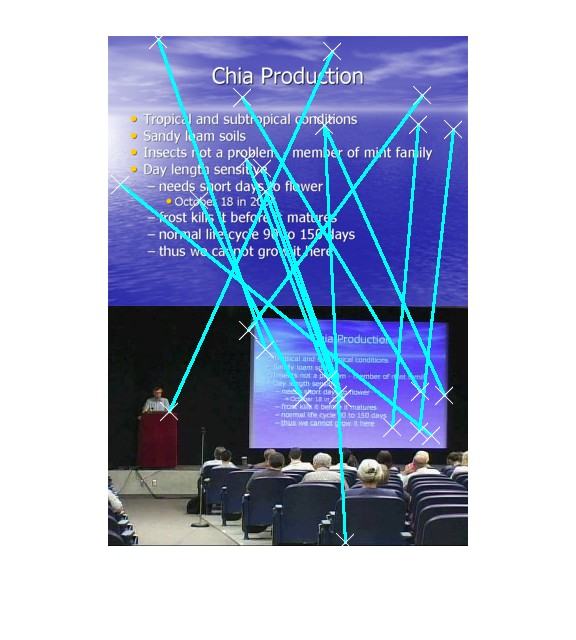
\includegraphics[width=3in]{new_figs/fCSF1x.jpg}}
		\caption{Slide/Frame 1 - First pair seems to perform the worst; on close inspection, the gradient (going from purplish tone to blue) on the slide is opposite to gradient on the frame. Therefore, multiple keypoints are matched opposite considering the water-like texture/background of the slide/frame.}
	\end{subfigure}
	\begin{subfigure}{0.4\textwidth}
	    {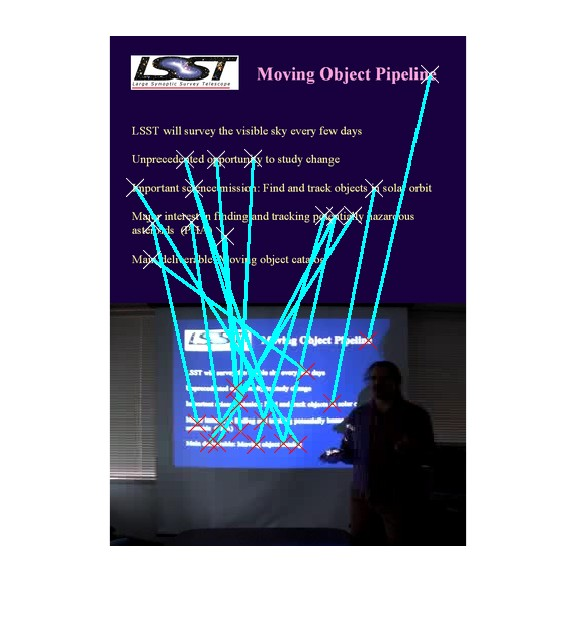
\includegraphics[width=3in]{new_figs/fCSF2x.jpg}}
		\caption{Slide/Frame 2 - Second pair performed better than the first. There are still some mis-matches, but we were happy to see the perfect matches like the end of word "pipeline", "in" in the third line, and so on.}
	\end{subfigure}
	\begin{subfigure}{0.4\textwidth}
	    {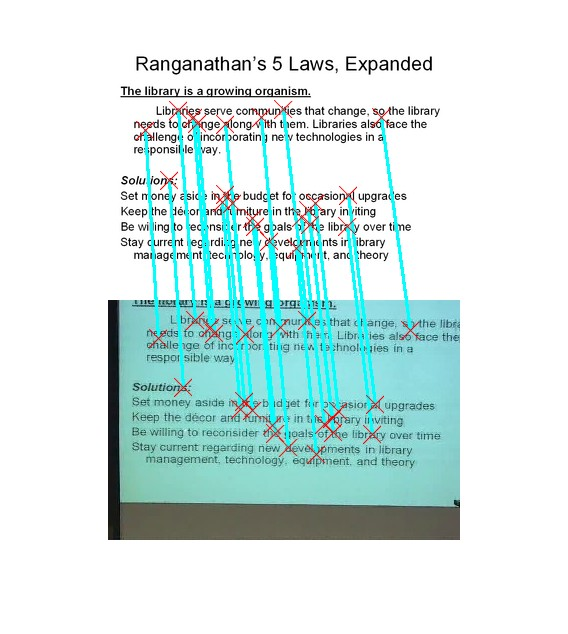
\includegraphics[width=3in]{new_figs/fCSF3x.jpg}}
	    \caption{Slide/Frame 3 -  Third pair performed the best.}
	\end{subfigure}
	\caption{ Figure showing the mapping of keypoints for the provided slide-frame pairs. These slide keypoints were estimated from the frame keypoints using the homography computed with RANSAC algorithm. We picked our keypoints based on the lowest Euclidean distance and were getting similar results using the distance between the matches as the angle between feature vectors.}
\label{fig:slideframeC}
\end{figure}
